\section{Gaussian Processes}
\label{gp}

Given a parameter space $\mathbb{X} \subset \mathbb{R}^m$ and an unknown, noisy cost function $f$ that is expensive to evaluate, we aim to find the solution to the minimization problem
\begin{align}
  x^* = \argmin_{x \in \mathbb{X}} f(x),
\end{align}
by iteratively choosing points to evaluate until a stopping criteria is met. Bayesian optimization, a sequential design strategy, computes a posterior distribution on possible objective functions given all previous evaluations and optimizes an acquisition function on this distribution to globally select the next value of $x$ to evaluate, typically in a way that carefully balances exploration and exploitation. The distribution over $f$ is modeled as a Gaussian process \citep{Rasmussen2006} $\mathbb{G}$, 
\begin{align}
  f \sim \mathbb{G}(\mu, \kappa), 
\end{align}
where $\mu : \mathbb{X} \rightarrow \mathbb{R}$ is a mean function typically set to zero, and $\kappa : \mathbb{X}\times \mathbb{X} \rightarrow \mathbb{R}$ is a covariance kernel that characterizes the correlation between different points in the domain. There are a number of options for covariance kernels, both stationary and non-stationary, but the most widely known is the squared exponential
\begin{align}
  \kappa(x_i, x_j \vert \theta) = \sigma_\theta^2 \exp(-\frac{1}{2}d^2(\frac{x_i}{l}, \frac{x_j}{l})),
\end{align}
with parameter $\theta = [\sigma_\theta^2, l]$ where $\sigma_{\theta}$ is a scalar, $l$ is either a scalar or vector of dimension $m$, and $d(x_i, x_j)$ is the Euclidean distance. The Matérn covariance kernel is a more generalized form of the squared exponential, defined as
\begin{align}
	\kappa(x_i, x_j \vert \theta) = \sigma_\theta^2\frac{2^{1-\nu}}{\Gamma(\nu)}(\sqrt{2\nu} d(\frac{x_i}{l}, \frac{x_j}{l}))^\nu K_\nu (\sqrt{2\nu} d(\frac{x_i}{l}, \frac{x_j}{l}))
\end{align}
with an additional scalar $\nu$ and $K_\nu$ is a modified Bessel function.
\section{GP Regression and Acquisition Functions}
\label{gp_acq}
By definition of a GP, any collection of points forms a multivariate normal distribution defined by $\mu$ and $\kappa$. Under this assumption, a posterior distribution given a set of training samples can be solved analytically. Formally, given some training samples $\mathbb{S} = \{(x_i, y_i)\}_{i=1}^n$, and assuming each sample follows a Gaussian noise model $y_i \sim f(x_i) + \mathcal{N}(0, \sigma_n^2)$, the posterior distribution at $x$ is Gaussian with mean $\bar{\mu}(x)$ and variance $\bar{\sigma}^2(x)$ evaluated as
\begin{gather}
  \bar{\mu}(x) = K(X, x)^T[K(X, X) + \sigma_n^2 I]^{-1}Y \\
  \bar{\sigma}^2(x) = \kappa(x, x\vert \theta) - K(X, x)^T[K(X,X) + \sigma_n^2 I]^{-1}K(X,x) \\
  K(X,x)_i = \kappa(x_i, x\vert \theta) \nonumber\\
  K(X,X)_{ij} = \kappa(x_i, x_j\vert \theta) \nonumber,
\end{gather}
where $X = \{x_i\}_{i=1}^n$ and $Y = \{y_i\}_{i=1}^n$. 
\begin{figure}[t]
\centering
\includegraphics[width=\textwidth]{gp_regression.png}
\caption{Sample GP Regression of a function using squared exponential and Matérn kernels.}
\label{fig:gp_regression}
\end{figure}

Given a Gaussian distribution at point $x$, an acquisition function captures how attractive that point is to sample next. A common choice of acquisition function is Expected Improvement (EI), which returns the expected reduction in cost over the best parameters observed so far. For the given GP model, EI can be computed in closed form: 
\begin{align}
  \begin{split}
  EI(x\vert \mathbb{S}) &= \int_\infty^\infty max(0, y^*-y)p(y\vert x)dy\\
    &= z\bar{\sigma}(x)\Phi(z) + \bar{\sigma}(x)\phi(z)
  \end{split}\\
  z &= \frac{y^* - \bar{\mu}(x) + \xi}{\bar{\sigma}(x)}\nonumber,
\end{align}
where $y^*$ is the best value observed so far and $\xi$ is a scaling parameter to adjust the tradeoff between exploration-exploitation \citep{Lizotte:2008:PBO:1626686}. The next point to evaluate is then chosen as $x^* = \argmax_{x} EI(x \vert \mathbb{S})$. Figure \ref{fig:ei} shows a few iterations of Bayesian Optimization on a sample function.

The choice of $y^*$ can be defined as the minimum observed value so far, the minimum $\bar{\mu}(x)$ under the current GP model over all previous observations, or some biased version thereof \citep{Lizotte:2008:PBO:1626686}. 

\section{Hyperparameter Optimization and Student-t Noise Model}
\label{gp_hyperparam}
The values of the hyperparameters in the kernel function are critical to determining the posterior distribution. Typically, these hyperparameters are tuned to sampled points with a maximum a posteriori (MAP) point estimate \citep{NIPS2012_4522,GPstuff}. Specifically, assuming our Gaussian noise model the MAP estimate is defined as
\begin{gather}
\argmax_{\theta, \sigma_n^2} \text{ } log P(\mathbb{S}\vert \theta, \sigma_n^2) + log P(\theta, \sigma_n^2)\\
=log \int p(Y\vert f, \sigma_n^2)p(f\vert X,\theta)df + log P(\theta, \sigma_n^2)\nonumber\\
= -\frac{n}{2}log(2\pi) - \frac{1}{2}log(K(X,X) + \sigma_n^2 I) - \frac{1}{2}Y^T(K(X,X) + \sigma_n^2 I)^{-1}Y + log P(\theta, \sigma_n^2)\nonumber
\end{gather}


\begin{algorithm}[t]
\caption{Bayesian Optimization Outline}
\label{alg:bayesopt}
\begin{algorithmic}
\State \textkeyword{Objective Function} $F(x)$
\State \textkeyword{Acquisition Function} $g(\mu, \sigma^2)$
\State \textkeyword{Specify Exploration Points } $\mathbb{E} = \{e_1, e_2, ..., e_n\}$
\State \textkeyword{Training Samples } $\mathbb{S}$
\For{i=1}{n}
  \State $\mathbb{S} = \mathbb{S} \cup \{e_i, F(e_i)\}$
\End
\While{t < T}
  \State Update GP Hyperparameters $\theta$
  \State Given $f(x\vert \theta, \mathbb{S}) \sim \mathcal{N}(\mu_x, \sigma_x^2)$,
  \State $x^* = \argmax_{x \in \mathbb{X}} g(\mu_x, \sigma_x^2)$
  \State $\mathbb{S} = \mathbb{S} \cup \{x^*, f(x^*)\}$
\End
\end{algorithmic}
\end{algorithm}


Instead of using a single point estimate, a full Bayesian approach would involve marginalizing out the hyperparameters through an MCMC approximation. This would be particularly beneficial in the case where the posterior is multi-modal or sensitive to small changes in hyperparameter values. Many sampling approaches have been proposed, and we refer the reader to \cite[Chapter~14]{barber2011bayesian} for a summary. 

The MCMC approach is also used in more complex noise models whose posterior distribution and marginal likelihood are no longer analytically tractable. \citet{NIPS2009_3806,Jylanki:2011:RGP:1953048.2078209} developed a more robust noise model based on the Student-t distribution to handle occurrences of large outliers in the collected data. The noise distribution follows
\begin{align}
p(y\vert f,\sigma_n^2,\nu) = \frac{\Gamma (\frac{\nu + 1}{2})}{\Gamma(\frac{\nu}{2})\sqrt{\nu\pi}\sigma_n})(1 + \frac{(y-f)^2}{\nu\sigma_n^2})^{\frac{-(\nu + 1)}{2}}
\end{align} 
where $\nu$ is a degrees of freedom hyperparameter. A Gibbs sampler can be performed through a hierarchical model where each training sample's output noise follows an independent inverse chi-squared distribution
\begin{align}
\begin{split}
y_i\vert f &\sim \mathcal{N}(f, V)\\
V &\sim \text{Inv-}\chi^2(\nu, \sigma_i^2),
\end{split}
\end{align}
with $\theta$ alternately sampled according to the Gaussian Process. Figure \ref{fig:mcmcvsmap} shows a comparison of the robust Student-t noise with the standard Gaussian noise. The majority of data points exhibit low variance, while some extreme outliers are also produced. While the Gaussian noise model treats each data point equally, the Student-t model is able to effectively pick out the outliers and recreate the underlying function.

\begin{figure}[t]
\centering
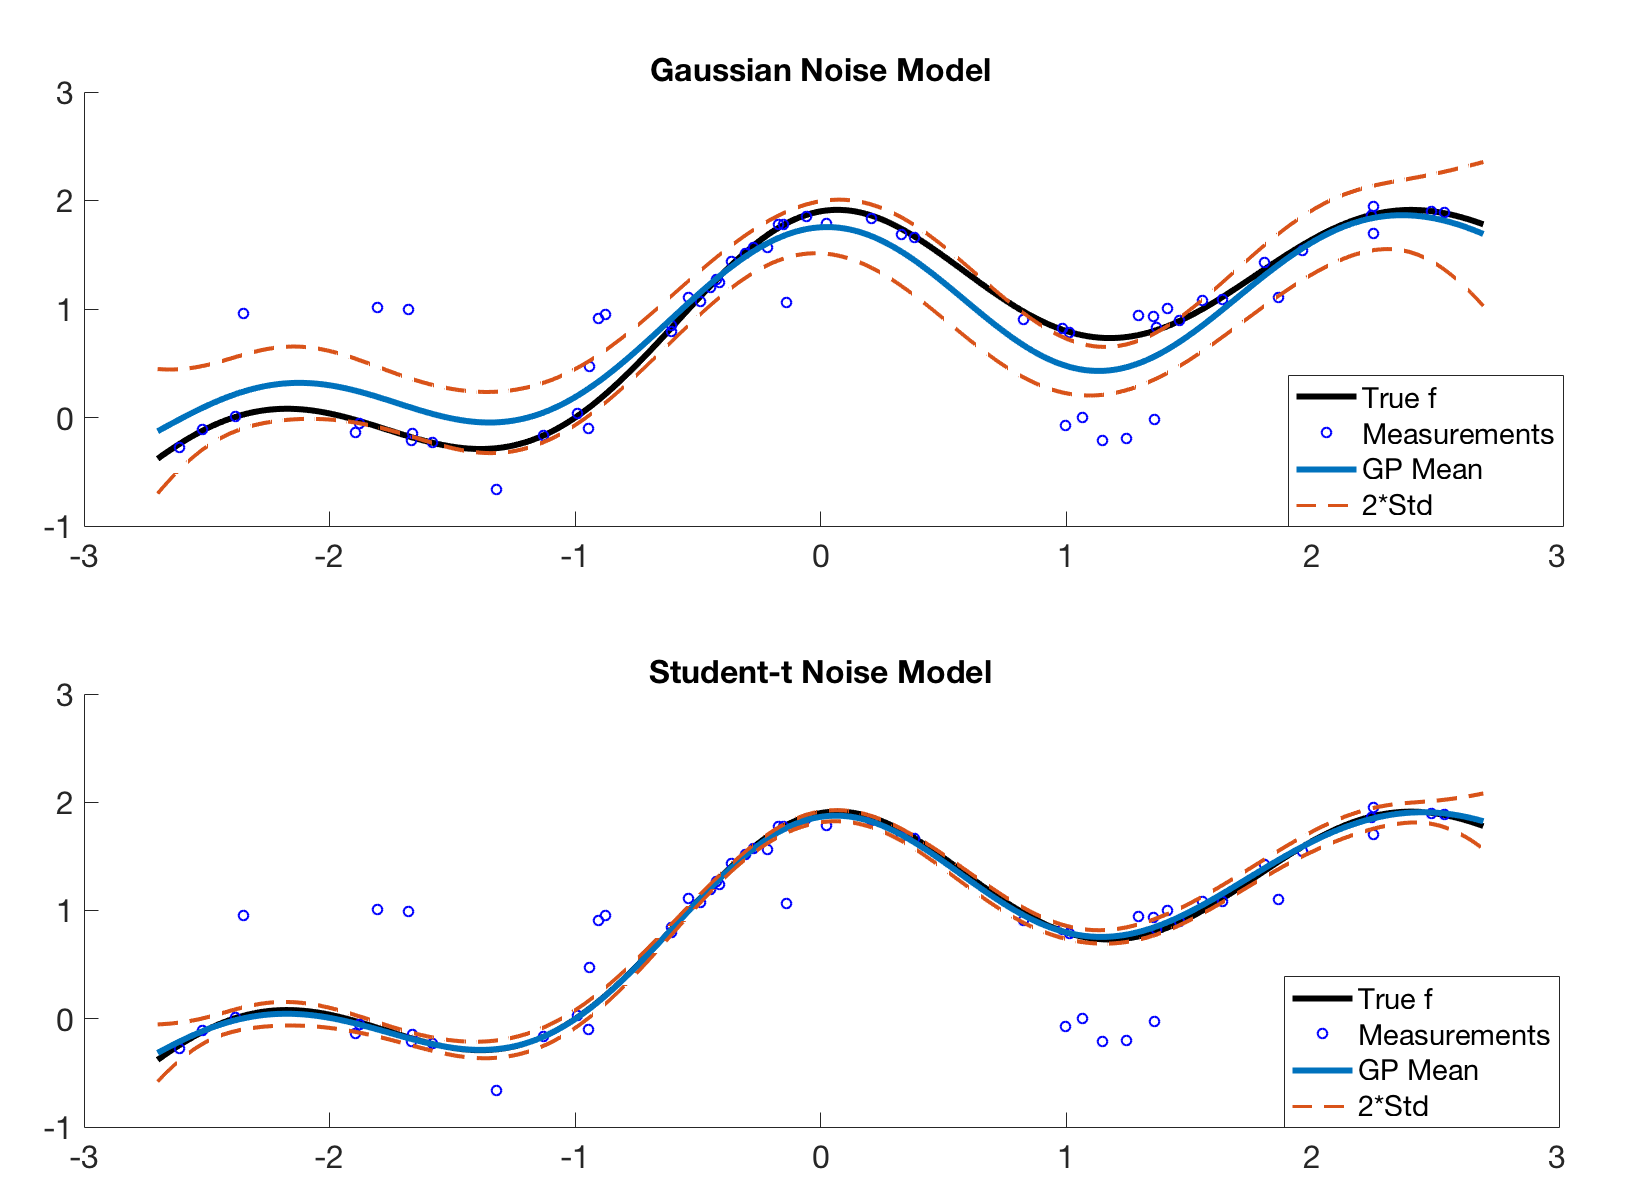
\includegraphics[width=\textwidth]{mcmcvsmap}
\caption{Gaussian MAP estimate vs. Student-t Gibbs Sampler. Data points added with Gaussian noise including some outliers with very high variance.}
\label{fig:mcmcvsmap}
\end{figure}

\section{Implementation}
There are a number of implementation choices relevant to HIL optimization. While the MCMC approach has shown to be more robust, GP regression scales linearly with the number of samples. Optimizing the acquisition function using a sufficient sample size is then increasingly expensive, taking on the order of minutes to evaluate. However, once a stopping condition is met the next parameter setting must immediately be communicated to the wearable device. In our implementation, we start an MCMC sampler concurrently with a new parameter evaluation. When the stopping condition is met, if the sampler has completed optimizing EI we use the returned parameter setting. Otherwise, we default to the MAP estimate to find the next parameter selection. There is then a tradeoff between the standard MAP estimate with a more robust MCMC sampler that uses one less training sample.

As Chapter \ref{ch:2} will discuss, the returned metabolic estimates have an associated variance; earlier stopping points exhibit a higher variance representing greater uncertainty for the estimated cost. The GP estimates may incorrectly inflate the best observed value if a number of parameter settings nearby are stopped early (see MAP estimate in Figure \ref{fig:mcmcvsmap} for $x\in(-2, -1)$). To appropriately weight the training samples based on their estimator variances, we fix separate noise hyperparameters corresponding to each sample. In the Gaussian noise model, the regression equation then becomes
\begin{align}
\begin{split}
  \bar{\mu}(x) &= K(X, x)^T[K(X, X) + \Sigma]^{-1}Y \\
  \bar{\sigma}^2(x) &= \kappa(x, x\vert \theta) - K(X, x)^T[K(X,X) + \Sigma]^{-1}K(X,x),
\end{split}
\end{align}
where $\Sigma$ is a diagonal matrix of entries $\{\sigma_i^2\}$ corresponding to scaled variance estimates of each data point \citep{Kersting:2007:MLH:1273496.1273546}. In the case of the MCMC model, each $y_i$ is defined independently with a noise parameter already. Figure \ref{fig:fixednoise} gives an example of the effect of fixed noise hyperparameters on the GP. Additionally, we define $y^*$ in Expected Improvement as the best mean estimate rather than the observed value. The best observed value is equally likely to be an outlier among a set of nearby points that were all measured for the full duration, so we base our decision on the variance-scaled Gaussian process estimates.

\begin{figure}[ht]
\includegraphics[width=\textwidth]{fixednoise.png}
\caption{Demonstration of the effect of fixing measurement noise. Using the same data from Figure \ref{fig:mcmcvsmap}, the noise associated with each data point is fixed and inversely proportional to the true accuracy - in effect telling the GP that the minority outliers are the more accurate values. This may arise in our stopping problem where a minimum is found (measured for the full duration, resulting variance is relatively low) and many nearby points are subsequently sampled and stopped early (resulting variances are very high).}
\label{fig:fixednoise}
\end{figure}